% !TeX encoding = UTF-8
\section{Fundamentals}
\subsection{Basic definitions in graph theory}
Before we start with the proofs of algorithm, let's give some useful definitions in graph theory:

\begin{definition}
A \textit{cycle $C$} in $G$ is a simple path $v_1, v_2, ..., v_n$, where $v_n = v_1$. In the \textbf{Figure 1}, $v_1v_2v_3v_4$ is a cycle.
\begin{figure}[H] %H为当前位置,!htb为忽略美学标准,htbp为浮动图形
\centering %图片居中
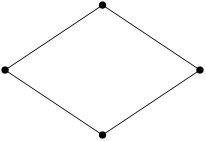
\includegraphics[width=0.4\textwidth]{figure/cycle.png} 
\caption{Cycle $C$} %最终文档中希望显示的图片标题
\label{figure} %用于文内引用的标签
\end{figure}
\end{definition}

\begin{definition}
When a connected graph can be drawn without any edges crossing, it is called \textit{planar}. When a planar graph is drawn in this way, it divides the plane into regions called \textit{faces}. \cite{Discrete_Mathematics} In \textbf{Figure 2}, $v_2v_3v_4v_5$ bounds a face. 
\begin{figure}[H] %H为当前位置,!htb为忽略美学标准,htbp为浮动图形
\centering %图片居中
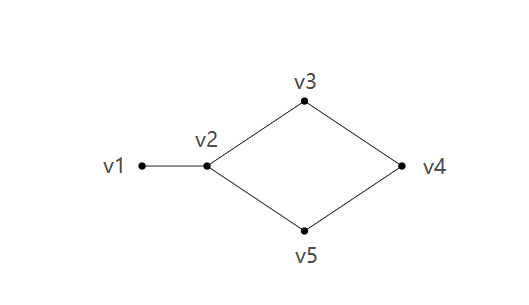
\includegraphics[width=0.5\textwidth]{figure/face.png} 
\caption{Face $F$} %最终文档中希望显示的图片标题
\label{figure} %用于文内引用的标签
\end{figure}
\end{definition}

\begin{definition}
A cycle $F$ is a \textit{facial cycle} in $G$ if it bounds a face in a component in $G$(possibly the outer face), regardless of whether $F$ itself is a face or not. \cite{dvorak2013threecoloring} Both cycles in \textbf{Figure 3} are facial cycle.
\begin{figure}[H] %H为当前位置,!htb为忽略美学标准,htbp为浮动图形
\centering %图片居中
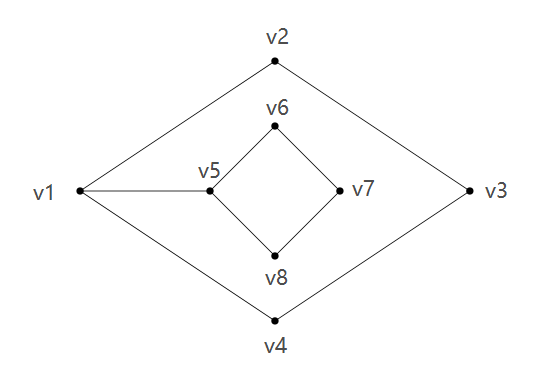
\includegraphics[width=0.5\textwidth]{figure/facialcycle.png} 
\caption{Both cycles $v_1v_2v_3v_4$ and $v_5v_6v_7v_8$ are facial} %最终文档中希望显示的图片标题
\label{figure} %用于文内引用的标签
\end{figure}
\end{definition}

\begin{definition}
A cycle $C$ in a connected graph $G$ is a \textit{separating cycle} if the deletion of $C$ from $G$ results in a disconnected graph. \cite{THOMASSEN197857} In the \textbf{Figure 4}, $v_1v_2v_3v_4$ is a separating cycle, because inside this cycle there are two more vertices $v_6, v_7$.
\begin{figure}[H] %H为当前位置,!htb为忽略美学标准,htbp为浮动图形
\centering %图片居中
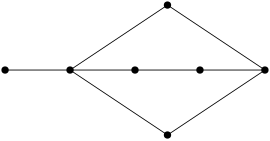
\includegraphics[width=0.4\textwidth]{figure/separating cycle.png} 
\caption{Separating cycle} %最终文档中希望显示的图片标题
\label{figure} %用于文内引用的标签
\end{figure}
\end{definition}

\begin{observation}
In a drawing of a graph, a cycle is either a facial face or a separating cycle.
\end{observation}

\begin{definition}
A vertex $v$ is \textit{incident} with an edge $e$ if $v \in e$; then $e$ is an edge at $v$. The two vertices incident with an edge are its endvertices or ends, and an edge joins its ends. \cite{diestel2010graph}
\end{definition}

\begin{definition}
In the plane, a face $f$ is \textit{the outer face}, if all vertices are contained inside in this face. 
\end{definition}

\begin{definition}
A \textit{open disk} is a cycle and everything inside it in a drawing of graph but not vertices on the bound. A \textit{closed disk} is a cycle and everything inside it in a drawing of graph including vertices on the bound.

\begin{figure}[H] %H为当前位置,!htb为忽略美学标准,htbp为浮动图形
\centering %图片居中
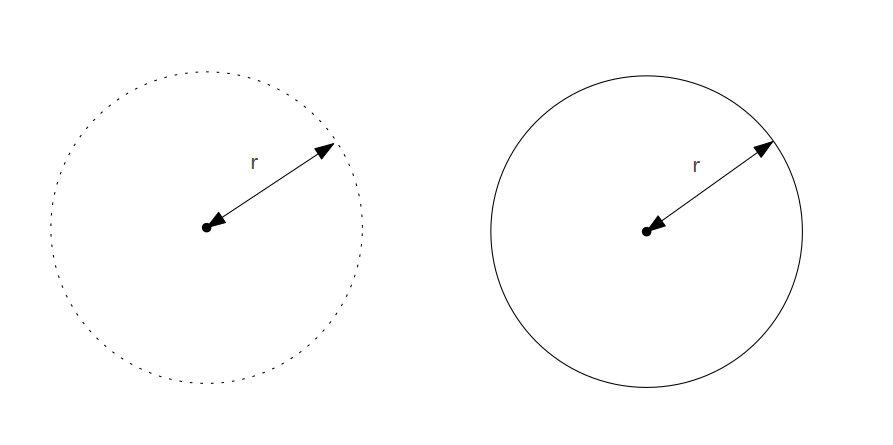
\includegraphics[width=0.7\textwidth]{figure/closeddisk.png} 
\label{figure} %用于文内引用的标签
\caption{Open and closed disks}
\end{figure}
\end{definition}

\begin{definition}
We say that $P = v_1v_2v_3...v_k$ is an \textit{induced path} in $G$ if $\forall v_iv_j \in E$ $\Longleftrightarrow$ $|i - j| = 1$.
\end{definition}

\subsection{The core idea}
After knowing these beneficial definitions, we will introduce five reducible configurations, also called \textit{multigrams}. With such multigrams, we can reduce the size of graph $G$ to have a smaller graph $G^{'}$ by identifying some vertices (see definition in the next section). Meanwhile, although we get a smaller graph $G^{'}$, its coloring can be reconstructed to the coloring of $G$ in constant time. The algorithm detects recursively such multigrams with certain constraints so that the size of graph will always get smaller each time until it's so simple to find the corresponding coloring. Next, according to the resulted coloring, we can reconstruct the coloring of its previous graph step by step. In the end, we'll get the proper coloring of the input graph. \footnote{Demonstration of the algorithm can be found in appendix}

